\section{Classification and placement}
\label{sec:intro:containerization}
Containerization technology has been introduced in BSD in the early 2000s and finally established in the Linux kernel in 2008 \cite{Souppaya:2017aa}. The resulting Linux containers(LXC's) are much more flexible and closer to the underlying host operating system than the classical full virtualization strategy from the 1960s. Figure \ref{fig:intro:diff_container_vm} shows the architectural difference between container and full virtualization. 

\begin{figure}[htbp]
 \centering
 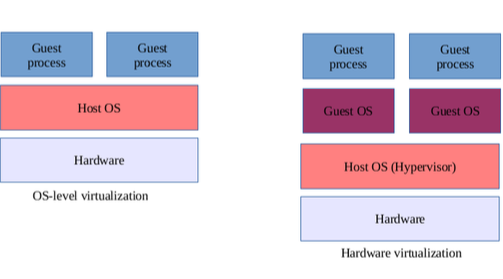
\includegraphics[width=0.7\textwidth]{gfx/examples/os_virt_diff}
 \caption{Difference between container and full virtualization}
 \label{fig:intro:diff_container_vm}
\end{figure}
The fact about the architectural difference leads to important facts.
A container is a lightweight alternative to full machine virtualization. In fact a container does not require as seen in \ref{fig:intro:diff_container_vm} a virtualized hardware. The container is just using and sharing the underlying kernel from the host. 

Containers themselves are basically operated as stateless and distinct units, which are usually provided and destroyed by an orchestrator or by hand. If updates are available, the containers are simply replaced. This enables developers and system engineers to make and push changes to apps at a much faster pace.

The immutability of containers also affects data persistence. Instead of mixing the app with the data used, containers emphasize the concept of isolation. Data persistence should not be achieved by simply writing to the container root file system, but by using external, persistent data stores such as databases or volumes. Data should be used outside the containers themselves, so that when a container is replaced by a new version, all data is still available for the new container.

From BSD's first rudimentary container approach with jails to Linux LXC's to Docker, native Linux features provide the functional foundation for encapsulation between host and deployed containers.
These necessary isolation and permissions concepts of a recent Linux system(Kernel version 5.3.11) are described in the next sections.